\chapter{Device capability modelling}
\label{DeviceCapabilityModelling}

\begin{flushright}{\slshape    
Whenever we capture the complexity of the real world in \\
formal structures, whether language, social structures, or \\
computer systems, we are creating discrete tokens for \\
continuous and fluid phenomena. In doing so, we are bound \\
to have difficulty. However, it is only in doing these things\\
 that we can come to understand, to have valid discourse,\\
 and to design.} \\ \medskip
    ---  Alan Dix
\end{flushright}


%\section{Describing devices: Device modelling}
%CC/PP, UAProf, FIPA
%While it is possible to determine a device's capabilities from its information shadows \cite{OReilly2009}, the capabilities modelled in the smart space are only those which are meaningful to share. 
%- dcs ontology
%- UWA, Delivery Context Ontology (relates to UAProf)

In order to share device capabilities with other devices in the environment, we require ways to describe these capabilities. While we have touched lightly on some of the techniques in the thesis so far, this chapter will focus in more detail on the current state-of-the-art, as well as how we extended these techniques to create a new way of modelling device capabilities using ontologies.

Most of the existing work on modelling interaction capabilities focuses on \ac{GUI} based techniques. 

\section{GUI-based techniques}

A \emph{universal user interface language} describes user interfaces that are rendered by mapping a description's device-independent interaction elements to a target platform's concrete interface objects \cite{Lee2006}. This allows developers to create the user interface in an abstract language without targeting a specific device. Examples of interface languages include \ac{UIML}, \ac{XIML}, \ac{PUC} and \ac{INCITS/V2 URC}. These languages allow devices to determine the most suitable presentation based on a predefined set of abstract user interface components.

\ac{UIML} maps interface elements to target UI objects using a styling section, resulting in one styling section per target device type. However, it does not include a vocabulary to describe more abstract widgets \cite{Zimmermann2007}. \ac{PUC} describes device functions in terms of state variables and commands, with a grouping mechanism used for placement of UI objects. The \ac{INCITS/V2 URC} standards define a generic framework and an XML-based user interface language to let a wide variety of devices act as a remote to control other devices, called targets.

\emph{User interface remoting} uses a remote interface protocol that relays I/O events between an application and its user interface. The user interface resides on a remote platform instead of on the device itself. The \ac{UPnP} \ac{RUI}, that forms part of the \ac{UPnP} AV standard,  belong to this category. \ac{UPnP} \ac{RUI} follows the Web server-client model, where the controller acts as a remote user interface client, and the target, acting as a remote user interface server, exposes a set of user interfaces \cite{UPnPForum}.

CEA-2014, that builds on the \ac{UPnP} \ac{RUI} interface, uses a matchmaking process for a controller device to select a user interface protocol that is supported by the controller platform \cite{Zimmermann2007}. Supported protocols include AT\&T \ac{VNC} and Microsoft \ac{RDP}. \ac{VNC} uses the \ac{RFB} protocol to send pixels and event messages between devices. 

Universal user interface languages and user interface remoting are orthogonal approaches \cite{Lee2006}. User interface remoting might be used in parallel with device-independent user interface languages.

%\marginpar{Current remote user interfaces are device-oriented rather than task-oriented. CEA-2018, discussed earlier in Section \ref{cea2018}, tries to solve this problem by using task model representations.}



% Lee2006 also describes uJuni and INCITS / V2 URC

In this thesis we are more interested in tangible interactions in ubiquitous computing environments, instead of the usual \ac{GUI}-based solutions. Smart environments need not only descriptions of \ac{GUI}-based input/output, but also descriptions of the physical input/output capabilities, hardware capabilities, network capabilities and other characteristics of smart objects. The first attempt to define a vocabulary that conveys these device characteristics was the W3C \ac{CC/PP}\footnote{http://www.w3.org/Mobile/CCPP/}. Other approaches to describe device characteristics that are not \ac{GUI} specific are described in the next section.

\section{Non-GUI techniques}

\subsection{UAProf}

The WAP Forum's \ac{UAProf} specification is an \ac{RDF}-based schema for representing information about device capabilities.\marginpar{W3C's \ac{CC/PP} is also an \ac{RDF}-based schema.} UAProf is used to describe the capabilities of mobile devices, and distinguishes between hardware and software components for devices.

%start africon
%The User Agent Profile (UAProf) specification, used to describe the capabilities of mobile devices, distinguishes between hardware and software components for devices, but the descriptions of interaction capabilities are very limited. 

For example, in the Nokia 5800 XpressMusic UAProf profile\footnote{nds1.nds.nokia.com/uaprof/Nokia5800d-1r100-2G.xml
}, its interaction capabilities are described as follows:

\begin{itemize}
	\item \texttt{PhoneKeyPad} as \texttt{Keyboard}
	\item 2 as \texttt{NumberOfSoftKeys}
	\item 18 as \texttt{BitsPerPixel}
	\item 360x640 as \texttt{ScreenSize}
	\item Stereo as \texttt{AudioChannel}
\end{itemize}

Other user interaction capabilities are defined in a Boolean fashion of yes/no, e.g. \texttt{SoundOutputCapable}, \texttt{TextInputCapable}, \texttt{Voice\-Input\-Capable}.
%end africon

\subsection{Universal Plug and Play (UPnP)}
\label{UPnP}

\ac{UPnP} with its device control protocols is one of the more successful solutions\footnote{http://upnp.org/sdcps-and-certification/standards/sdcps/} to describing device capabilities. However, it only allows for the definition of one level of tasks \cite{Niezen2010}.

\ac{UPnP} was developed to support addressing, discovery, eventing and presentation between devices in a home network, and the current version (1.1) was released as the ISO/IEC 29341 standard in 2008. It consists of a number of standardised \acp{DCP} - data models that describe certain types of devices. The \acp{DCP} that have been adopted by industry include audio/video, networking and printers. \acp{DCP} for low power and home automation have not yet been adopted.

\ac{DLNA} is a complete protocol set around \ac{IP} and \ac{UPnP}, where to be certified for \ac{DLNA}, a device needs to have \ac{UPnP} certification first. This protocol set was developed mainly to increase interoperability between \ac{AV} equipment in the home. It achieves this by limiting the amount of options available in the original protocol standards.\marginpar{In an IEEE ComSoc online tutorial entitled \emph{Consumer Networking Standardizations}, Frank den Hartog from TNO stated that ``DLNA has been a major effort to get computer people to talk to consumer electronics people''.}

When describing the capabilities of a smart object, not only the interaction capabilities are important, but also the device states. With \ac{UPnP}, two types of documents are used to describe device capabilities and states. A \emph{device description document} describes the static properties of the device, such as the manufacturer and serial number \cite{Jeronimo2009}. \ac{UPnP} describes the services that a device provides in \emph{service description documents}. These XML-based documents specify the supported actions (remote function calls) for the service and the state variables contained in the service. 

The state variable descriptions are defined in a similar way to how we define our interaction primitives, with a unique name, required data type, optional default value and recommended allowed value range. The \ac{UPnP} Forum has defined their own custom set of data types, with some similarity to the XML Schema data types used by \ac{OWL} 2. As an example, consider a state variable to describe the darkness of a piece of toast, where \texttt{ui1} is defined as an unsigned 1-byte integer:

\begin{minted}{xml}
	
<stateVariable sendEvents="no">
	<name>darkness</name>
	<dataType>ui1</dataType>
	<defaultValue>3</defaultValue>
	<allowedValueRange>
		<minimum>1</minimum>
		<maximum>5</maximum>
		<step>1</step>
	</allowedValueRange>
</stateVariable>

\end{minted}

The \texttt{sendEvents} attribute is required for all state variable descriptions. If set to \texttt{"yes"}, the service sends events when it changes value. Event notifications are sent in the body of an HTTP message and contain the names and values of the state variables in XML. 

Let us consider these device states in terms of user interaction. There are four key concepts in an interaction - actions, states (internal to the device), indicators, and modes (physically perceivable device states) \cite{Thimbleby2007}. The user performs actions, which change the device state, which in turn control indicators (augmented feedback). Users may not know exactly which state or mode a system is in. \marginpar{Our approach to modelling devices states and state transitions using \acp{FSM} is described in Section \ref{fsmexample}. } If we want to fully capture the capabilities of the device, we need to specify the device states, the transitions between these states, the interaction primitives which can cause these state changes, as well as the default and current states of the device. When this device is then connected to another device, we also need a way to communicate state changes to the other device.


%end TiiS


\subsection{SPICE DCS}
\label{spice}
The \ac{SPICE} Mobile Ontology\footnote{http://ontology.ist-spice.org/} allows for the definition of device capabilities in a sub-ontology called \ac{DCS} \cite{Villalonga2009}. A distinction is made between device capabilities, modality capabilities and network capabilities. While the ontology provides for a detailed description of the different modality capabilities, e.g. being able to describe force feedback as a \texttt{Tactile\-Output\-Modality\-Capability}, there are no subclass assertions made for other device capabilities. Most physical characteristics of the devices are described via their modality capabilities, e.g. a \texttt{screenHeight} data property extends the \texttt{VisualModalityCapability} with an integer value, and the \texttt{audio\-Channels} data property is also related to an integer value with \texttt{Acoustic\-Modality\-Capability}. The input format of audio content is described via the \texttt{Acoustic\-Input\-Modality\-Capability} through an \texttt{inputFormat} data property to a string value.

%It is not clear whether the modality capabilities should be used to describe the actual content that may be exchanged or the user interaction capabilities. As an example, if a device has an \texttt{Acoustic\-Output\-Modality\-Capability}, it is not clear whether the device can provide user interaction feedback (e.g. in the form of computer-generated speech or an audible click), or that the device has a speaker.




\section{Registering devices on startup}

Based on this existing work, we now look at our approach to registering device functionalities, as well as how we identify devices in the digital and physical domain.

On device startup, the smart object registers its digital and physical identification information (e.g. RFID tag or IP address) and its functionality with the SIB, and then subscribes to new connections and events as shown in Figure \ref{connectorsibSequence}.


\begin{figure}[bth]
\begin{msc}
msc {
	//hscale = "1.5";
	
    A [label="Smart Object A"],sib [label="SIB"], connector [label="Connector Object"]; // B [label="Smart Object B"];
	A->sib [label="Register identification info"];
	A->sib [label="Register functionality"];
    A->sib [label="Check for existing connections"];
    --- [label="If connection exists", ID=1];
    sib->A [label="Connection exists to B"];
    A->sib [label="Subscribe to source events"];
    --- [label="End if", ID=1];
    A->sib [label="Subscribe to connection changes"];
    A=>A [label="Waits for new event or connection"];
    connector->sib [label="New connection from B to A"];
    sib->A [label="New connection"];
    A->sib [label="Subscribe to source events from A"];
    A=>A [label="Waits for new event or connection"];
    connector->sib [label="Connection removed from B to A"];
    sib->A [label="Connection removed"];
    A->sib [label="Unsubscribe from source events"];
    A=>A [label="Waits for new event or connection"];
}
\end{msc}
        \caption{Startup sequence between smart object and SIB}
        \label{connectorsibSequence}
\end{figure}

\marginpar{The startup sequence contains instances of the blackboard and publish/subscribe patterns described in Section \ref{pubsubblackboard}.} This sequence is the same for all smart objects that connect to the \ac{SIB}, and should be implemented in every \ac{KP} that uses our approach. You might notice some parallels between the concept of a \ac{SIB} and the Microsoft Windows Registry. The Registry is used to store configuration information of software applications on a single device, while the \ac{SIB} is used (among other things) to store device functionality descriptions of a system of devices. However, compared to the Windows Registry, which is a basic hierarchical key-value store, the triple store and reasoning engine used in the \ac{SIB} provide a number of advantages, including subsumption testing, consistency checking and the ability to use restrictions to constrain data instances.\marginpar{Subsumption testing, consistency checking and restrictions are discussed in more detail in Section \ref{owlreasoning}.} This means we can use reasoning to verify the consistency and stability of the data in the \ac{SIB}.

We now discuss the first two steps of the sequence diagram in Figure \ref{connectorsibSequence}, registering identification and functionality, in more detail.

\subsection{Identifying devices}

In order to discover a device's capabilities, it is first necessary to be able to uniquely identify the device. Today it is common to identify groups of products using barcodes and other numbering systems. Before ubiquitous computing, only expensive things such as precious metals, currency, or large machines were individually identified with any regularity \cite{Kuniavsky}. New tracking technologies like \ac{RFID} tags and smart cards allow us to link a unique identification number to a specific physical product, like a smart phone that identifies a specific person to the phone network. IPv6, an extension to the Internet Protocol standard, allows us to identify approximately $3.4 \times 10^{38} $ objects in the digital domain.

% The significance of technologies like \ac{RFID} is that they offer a way to endow physical objects with an \emph{information shadow} \cite{Greenfield2006}. An information shadow describes the digital information that is tied to a specific product. \marginpar{Amazon.com for example, use their \ac{ASIN} to uniquely identify every product they sell.} In Bruce Sterling's book about ubiquitous computing and design, Shaping Things \cite{Sterling2005}, he uses the example of a wine bottle to describe these kinds of objects. 
% 
% Wine bottles have easily findable identifiers that link to their information shadows, usually consisting of a large amount of user-generated content. In addition to the metadata that is on the label, like the year when it was bottled, or the grapes that were used, information shadows provide information ``about the people and processes that made the bottle and its contents''. He argues that the wine's carefully designed information aspects, like the web page and bar code, permanently change people's relation to wine. The question now becomes: How do create and link these physical and digital identities in ubiquitous computing environments?

% Possible TODO "unique naming" papers on Mendeley

Mavrommati et al \cite{Mavrommati2004} linked an XML-based description of an object's properties, services and capabilities with an artefact ID. This alphanumeric ID is mapped to a namespace-based identification scheme, using a similar process to the one used for computer MAC addresses.

Tungare et al \cite{Tungare2007} identified an information object in their Syncables framework, used to migrate task data and state information across platforms, via a \ac{URI}. They used the structure 

\begin{verbatim}
sync://<info-cluster-id>/<collection>/<type>/<path>/<object-name>	
\end{verbatim}

where the information cluster is the set of all devices a user interacts with during the course of a day. Each of the devices in an information cluster ``offers a unique set of affordances in terms of processing capabilities, storage capacities, mobility constraints, user interface metaphors, and application formats''.

Most service discovery mechanisms, for example those used by \ac{UPnP}, assume the user will use the Internet to establish connections \cite{Jeronimo2009}. However, when we are in close proximity to things, we can address these things by pointing at them, touching them or by standing near them, instead of having to search or select them through a \ac{GUI}.

Olsen et al. \cite{Olsen2001} used the domain name or IP address of a software client associated with a device to identify it, and a URL to identify services associated with a specific device. A user was associated with a URL used for that user's current session. The physical user was identified using a Java ring, with a small Java virtual machine running on the ring's microcontroller. 

% Possible TODO Rekimoto TranSticks colour coding
% Possible TODO Hinckley bumping devices

% \cite{Olsen2001} recognised that in ubiquitous computing scenarios it is important to be able to identify where the user is located relative to devices, and focused on \emph{identity} and \emph{adjacency} instead of geometry. A global geometry model is one way of solving the problem, but is quite complex. It may not be necessary to know exactly where the user is, but only what devices they are near.


O'Reilly and Battelle \cite{OReilly2009} argue that formal systems for adding a priori meaning to digital data are actually less powerful than informal systems that extract that meaning by feature recognition. They think that we will get to an Internet of Things via a ``hodgepodge of sensor data, contributing, bottom-up to machine-learning applications that gradually make more and more sense of the data that is handed to them''. As an example, consider that using smart meter data to extract a device's unique energy signature, it is possible to determine the make and model of each major appliance.

Jeff Jonas's work on \emph{identity resolution} uses algorithms that semantically reconcile identities \cite{Segaran2009}. His \ac{NORA} technology is a \emph{semantically reconciled and relationship-aware directory} that is used by the Las Vegas gaming industry to identify cheating players within existing records. A semantically reconciled directory recognises when a newly reported entity references a previously observed entity.

%\marginpar{``I think the only way forward is going from applying algorithms to individual transactions, to first placing information in context--pixels to pictures--and only applying algorithms after one sees how the transaction relates to the other data. It's the only way that I can see that it's going to close this sense-making gap.'' -- Jeff Jonas}

We agree that waiting until every object has a unique identifier for the Internet of Things to work is futile. However, the Semantic Web was designed with this problem in mind. We can use a \ac{URI} to identify an entity we are talking about. Different people will use different \acp{URI} to describe the same entity. We cannot assume that just because two \acp{URI} are distinct, they refer to the same entity \cite{Allemang2011}. This feature of the Semantic Web is called, the \emph{Non-unique Naming Assumption}. When using \ac{OWL}, it is necessary to assert that individuals are unique using the \texttt{owl:allDifferent} or \texttt{owl:differentFrom} elements. Individuals can be inferred to be the same, or asserted using \texttt{owl:sameAs}. For \ac{OWL} classes and properties, we can use \texttt{owl:equivalentClass} and \texttt{owl:equivalentProperty}.

\begin{figure}[bth]
	\begin{center}
	\digraph[scale=0.6]{identification}{
		rankdir=LR;
		string [label="xsd:string", shape="plaintext"];
		SmartObject -> Identification [label="hasIdentification"];
		Identification -> string [label="idValue"];
		Identification -> IDType [label="ofIDType"];
	}
	\end{center}
	\caption{Modelling identification in the ontology}
	\label{identification}
\end{figure}

We modelled the identification of smart objects as shown in Figure \ref{identification}. An example of how the Squeezebox \ac{KP} can be linked to both its IP address and \ac{RFID} tag is shown below:

\begin{minted}{turtle}
SqueezeboxKP a SmartObject .
SqueezeboxKP hasIdentification id1234 .
SqueezeboxKP hasIdentification id4567 .
id1234 ofIDType IPAddress .
id1234 idValue "192.168.1.4:1234" .
id4567 ofIDType RFID_Mifare .
id4567 idValue "12AB45CD67EF" .
\end{minted}

\subsection{Registering a device's functionality}

In the first design iteration we used a very simple approach to modelling the capabilities of devices, where \texttt{provides} and \texttt{consumes} properties linked smart objects to the names of the capabilities. During the later design iterations we modelled capabilities as functionalities of a device instead.\marginpar{Examples of \texttt{provides} and \texttt{consumes} were shown in Section \ref{OntologyDesign1}.}

To register the functionality of a device such as the Squeezebox internet radio, we can use the following triples:

\begin{minted}{turtle}
squeezeboxKP a SmartObject .
squeezeboxKP functionalitySource Alarm .
squeezeboxKP functionalitySink Alarm .
squeezeboxKP functionalitySink Music .	
\end{minted}

This indicates that the device is capable of acting both as a source and as a sink for \texttt{Alarm} functionality, while it can act as a sink for \texttt{Music} functionality. Once these device capabilities are registered, we can use semantic reasoning to infer which devices can be connected to each other.



\section{Reasoning with device capabilities}
\label{ReasoningCapabilities}
A smart object can have one or more functionalities that can be shared with other smart objects. As shown in the previous section, we model a functionality as 

\begin{minted}{turtle}               
ie:Alarm a ie:Functionality .
ie:phone1 a ie:SmartObject .
ie:phone1 ie:functionalitySource ie:Alarm . 
\end{minted}

or in the case of modelling the functionality of a sink we use

\begin{minted}{turtle}               
ie:Music a ie:Functionality .
ie:speaker1 a ie:SmartObject .
ie:speaker1 ie:functionalitySink ie:Music . 
\end{minted}

To infer that two devices can be connected based on functionality as shown in Figure \ref{canConnectTo}, we use an \ac{OWL} 2 property chain:\\

\noindent
functionalitySource~\ensuremath{\circ}~isFunctionalityOfSink~\ensuremath{\sqsubseteq}~canConnectTo\\%\footnote{The concatenation of two relations $R$ and $S$ is expressible by $R \circ S $, while $ R \sqsubseteq S$ indicates that $R$ is a subset of $S$ }\\
\marginpar{A similar method was used to match media types in Section \ref{SemanticMatching}.}
\noindent
where we use \texttt{isFunctionalityOfSink}, the inverse property of \texttt{func\-tion\-al\-i\-ty\-Sink}, to be able to create the property chain.

\begin{figure}[bth]
        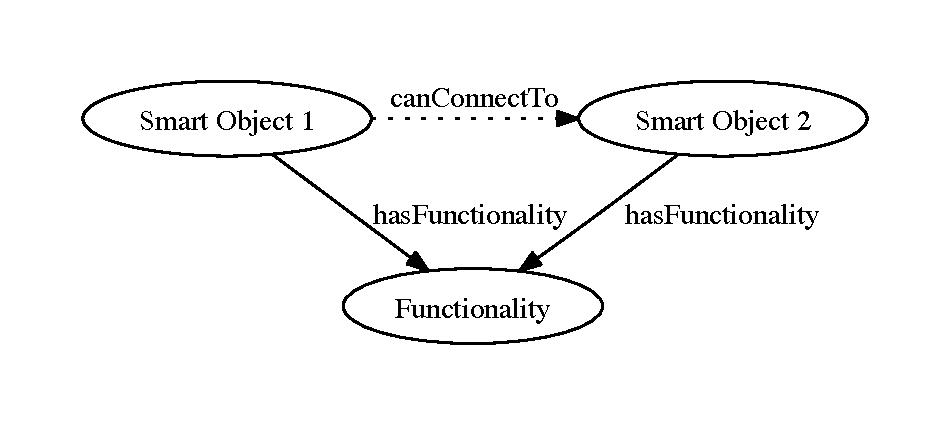
\includegraphics[width=\linewidth]{canConnectTo}
        \caption{Inferring connection possibilities based on functionality}
        \label{canConnectTo}
\end{figure}

To prevent a smart object from having a \texttt{canConnectTo} relationship to itself (which will be the case for semantic transformers), the relationship is defined to be irreflexive. Inferring indirect connection possibilities is also possible with a property chain:\\

\noindent
canConnectTo~\ensuremath{\circ}~canConnectTo~\ensuremath{\sqsubseteq}~canIndirectlyConnectTo

%When the \texttt{connectedTo} relationship is inserted, we also want to infer a \texttt{indirectlyConnectedTo} relationship. It turns out that this is something that is not expressible in OWL. (Q2336 (02/02/2012))


\subsection{Representing functionalities as predicates}
\label{predicateFunctionality}
If we want to model the common functionalities between two smart objects, we can use the n-ary ontology design pattern \cite{Noy2006}.\marginpar{Ontology design patterns are discussed in Chapter \ref{OntologyEngineering}.} Unfortunately, this is not intuitively readable from its ontological representation, as shown in the top half of Figure \ref{naryFunctionality}. The representation looks complicated and is difficult to read. On the other hand, we can also directly infer the matched functionalities as predicates, instead of using n-ary representations. The result can be represented using three triples instead of nine triples, and it is also more intuitively understandable, as shown in the bottom half of Figure \ref{naryFunctionality}.

\begin{figure}[bth]\centerline{
        %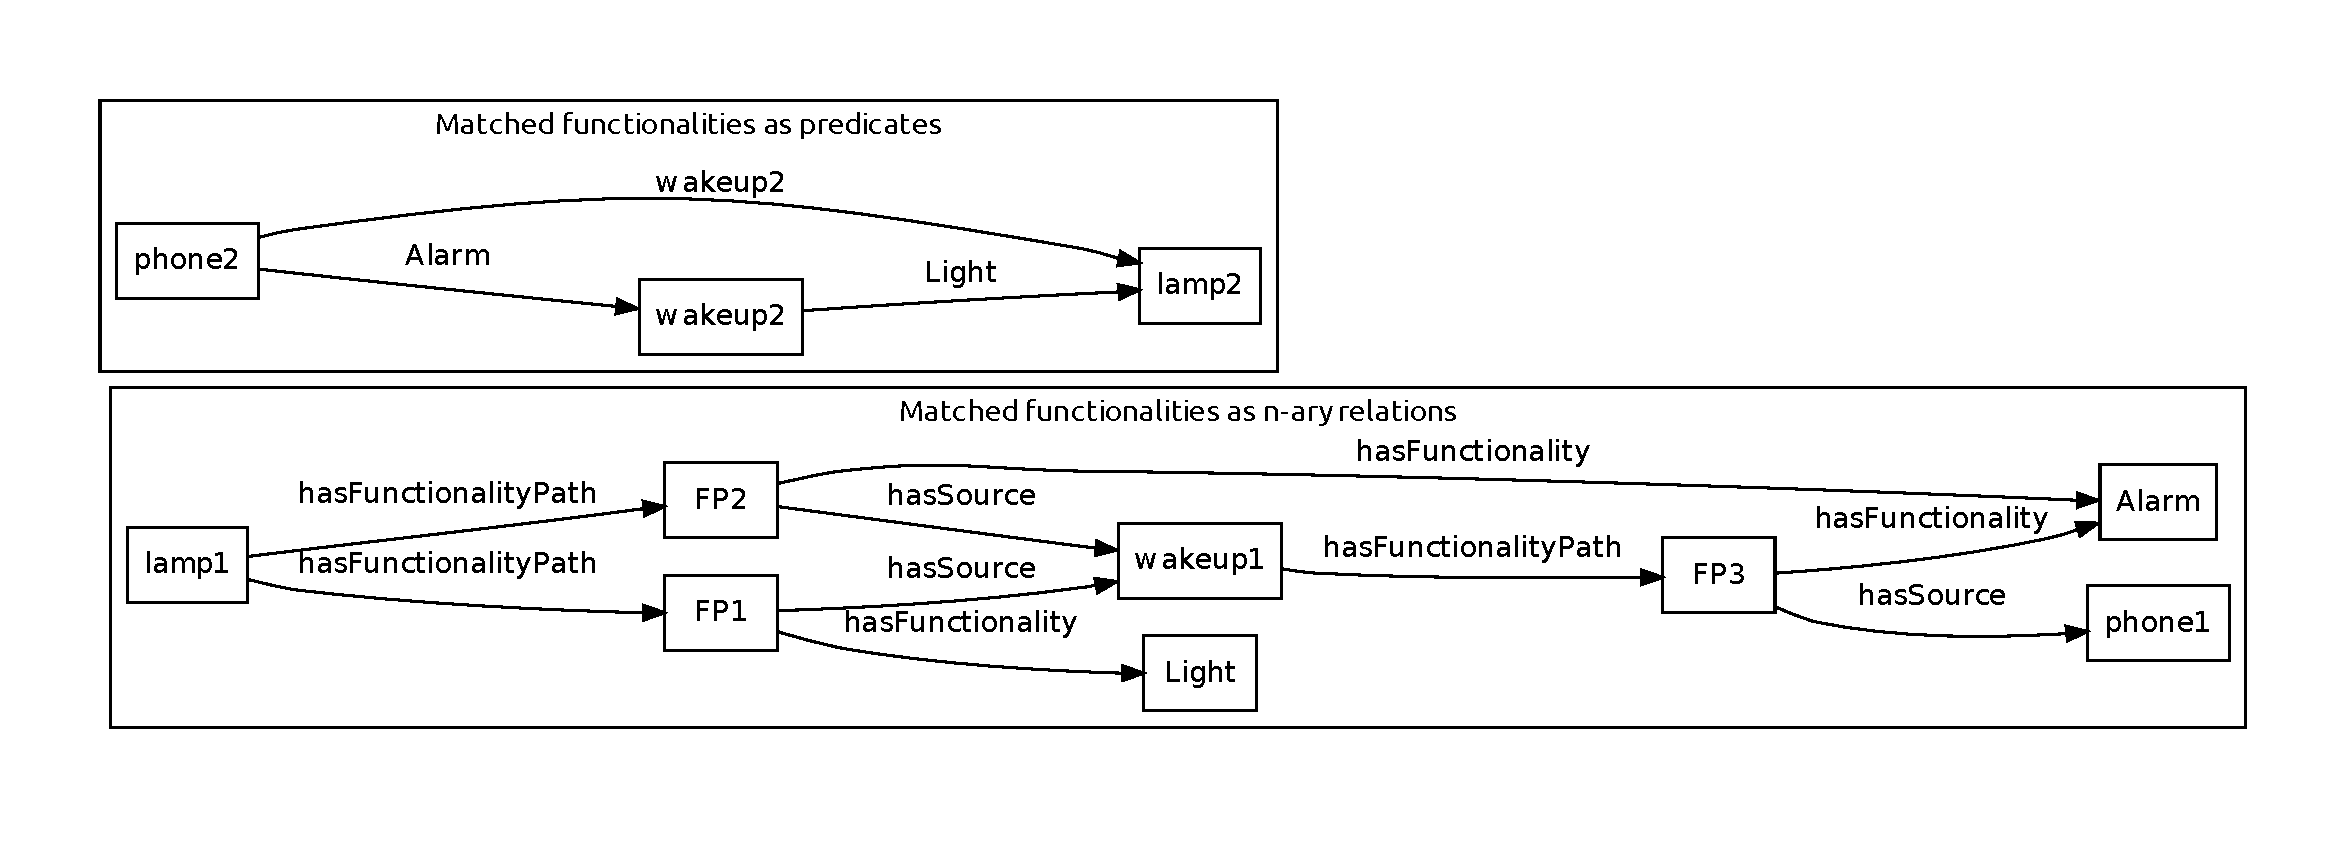
\includegraphics[width=450px]{naryFunctionality}
	\digraph[scale=0.45]{g}{
		rankdir=LR;
		compound=true;
		%fontname="Ubuntu";
		node [shape = box];
		lamp1->phone2 [style=invis]; % to ensure cluster0 is first
		subgraph cluster0 {
		label = "Matched functionalities as n-ary relations";
		lamp1 -> FP1 [label="hasFunctionalityPath"];
		FP1 -> Light [label="hasFunctionality"];
		FP1 -> wakeup1 [label="hasSource"];
		lamp1 -> FP2 [label="hasFunctionalityPath"];
		FP2 -> Alarm [label="hasFunctionality"];
		FP2 -> wakeup1 [label="hasSource"];
		wakeup1 -> FP3 [label="hasFunctionalityPath"];
		FP3 -> Alarm [label="hasFunctionality"];
		FP3 -> phone1 [label="hasSource"];
		}
		subgraph cluster1 {
		label = "Matched functionalities as predicates";
		phone2 -> wakeup2 [label="Alarm"];
		wakeup2 -> lamp2 [label="Light"];
		phone2 -> lamp2 [label="wakeup2"];
		}
	}
	}	
        \caption{Representing matched functionalities: N-ary relations versus predicates}
        \label{naryFunctionality}
\end{figure}

Representing an individual as a predicate is not valid in OWL 2 DL and places the ontology into OWL 2 Full. However, since we are using an OWL 2 RL/RDF Rules reasoning mechanism, this is not an issue. Thus we choose to use predicates instead of n-ary relations, and so we do not stay within OWL 2 DL. We can easily infer this relation using a \ac{SPIN} rule:

\begin{minted}{sparql}
CONSTRUCT {
    ?this ?functionality ?sink .
}
WHERE {
    ?this :functionalitySource ?functionality .
    ?sink :functionalitySink ?functionality .
}
\end{minted}

where \texttt{?this \ensuremath{\equiv} SmartObject}. For example, if we have a phone and a speaker with a common \texttt{Music} functionality, defined as

\begin{minted}{turtle}
:phone1 :functionalitySource :Music .
:speaker1 :functionalitySink :Music .
\end{minted}

the above \ac{SPIN} rule will infer

\begin{minted}{turtle}
	:phone1 :Music :speaker1 .
\end{minted}

such that the functionality itself is represented as a predicate. For a semantic transformer, which is indirectly connected to smart objects, we need an additional \ac{SPIN} rule:

\begin{minted}{sparql}
CONSTRUCT {
    ?source ?this ?sink .
}
WHERE {
    ?source :canIndirectlyConnectTo ?this .
    ?this :canIndirectlyConnectTo ?sink .
}
\end{minted}

where \texttt{?this \ensuremath{\equiv} SemanticTransformer}. This infers the semantic transformer itself as the relation between the source and the sink, since it transforms the original functionalities. For example, using the smart objects in Figure \ref{naryFunctionality}, if we have 

\begin{minted}{turtle}
	:phone2 :functionalitySource :Alarm .
	:wakeup2 :functionalitySink :Alarm .
	:wakeup2 :functionalitySource :Light .
	:lamp2 :functionalitySink :Light .
\end{minted}

and using the two property chains from Section \ref{ReasoningCapabilities}, we can infer that

\begin{minted}{turtle}
	:phone2 :canConnectTo :wakeup2 .
	:wakeup2 :canConnectTo :lamp2 .
	:phone2 :canIndirectlyConnectTo lamp2 .
\end{minted}

If we then apply the \ac{SPIN} rule defined above we can infer that 

\begin{minted}{turtle}
	:phone2 :wakeup2 :lamp2 .
\end{minted}

where the semantic transformer itself becomes the predicate between the two smart objects, signifying the possibility of having wakeup service functionality between the two objects.


How can we provide feedback or feedforward to the user that these possible functionalities exist between smart objects? This can be done using the feedback capability of the Connector object and the feedback capabilities of the devices themselves. Just after the user scans the second device, and before the connection is actually made, feedback of the different possibilities for shared functionality can be provided to the user. 

\marginpar{The \texttt{dataValue} property of interaction events is discussed in more detail in Section \ref{InteractionEvents}.} 
When two devices can be connected directly, the Connector object creates a temporary connection from itself to the sink. This temporary connection is specified using the \texttt{temp\-Connected\-To} property, a sub-property of the \texttt{connectedTo} property. The Connector object generates a \texttt{PreviewEvent} with the matching functionality as \texttt{dataValue}.\marginpar{Preview events and the \texttt{tempConnectedTo} property were first discussed in Section \ref{section:augmentedFunctionalFf}.}  This triggers the sink to create a preview of the functionality described by the \texttt{Preview\-Event} and its \texttt{dataValue}.  When the sink completes the preview, it generates its own \texttt{PreviewEvent} to indicate that it has finished. The Connector object sees the sink's \texttt{PreviewEvent} and removes the temporary connection.

\begin{figure}[bth]
	\digraph[scale=0.6]{stPreview}{
		{rank=same; Source; ST [label="Semantic Transformer"]; Sink;}
		{rank=max; Connector}
		Connector->ST [label= "tempConnectedTo"];
		ST->Sink [label = "tempConnectedTo"];
		Source->ST [label = "canConnectTo", style="dotted"];
		ST->Sink [label = "canConnectTo", style="dotted"];
		Source->Sink [label = "canIndirectlyConnectTo", style="dotted"];
	}
	\caption{Temporary connections for \texttt{PreviewEvent} when semantic transformer is used}
	\label{stPreview}        
\end{figure}

However, when there is a semantic transformer between the source and the sink, the Connector object creates a temporary connection to the semantic transformer instead of the sink, in order to generate the appropriate \texttt{PreviewEvent}, as shown in Figure \ref{stPreview}. Keep in mind that the semantic transformer is a virtual object, and therefore only the preview functionality generated by the sink will be perceivable by the user.

The Connector object uses the inferred \texttt{can\-Indirectly\-Connect\-To} and \texttt{canConnectTo} properties to determine where to insert the \texttt{temp\-Con\-nected\-To} properties. After inserting the \texttt{temp\-Con\-nected\-To} properties, the Connector object generates a \texttt{Pre\-view\-Event}. Due to the \texttt{temp\-Con\-nected\-To} relationship between the Connector object and the semantic transformer, the semantic transformer responds to this event and also generates a \texttt{Pre\-view\-Event} with its own functionality as \texttt{data\-Value}. Due to the \texttt{temp\-Con\-nected\-To} relationship between the semantic transformer and the sink, the sink responds to the preview event of the semantic transformer and generates the appropriate preview of its functionality.

Now that we have a way to model the capabilities of devices and provide previews of their functionality, we can start looking at ways to represent the different kinds of events that are generated on these devices in the next chapter.